\chapter{Syntroduction}
\label{syntroduction}
\blfootnote{{\color{rug-red} \faInfoCircle}~~This chapter draws in part on the introductions to the following chapters.}

\begin{fancyquotes}[font=\small\itshape]
It is interesting to contemplate an entangled bank, clothed with many plants of many kinds, with birds singing on the bushes, with various insects flitting about, and with worms crawling through the damp earth, and to reflect that these elaborately constructed forms, so different from each other, and dependent on each other in so complex a manner, have all been produced by laws acting around us.
\end{fancyquotes}

\begin{flushright}
    — Charles Darwin, \textit{On the Origin of Species} (1859)
\end{flushright}

\dropcap{C}harles Darwin's seminal work, \textit{On the Origin of Species}, published in 1859, introduced the scientific theory that populations evolve over generations through a process of natural selection. This theory was revolutionary at the time, providing a unifying explanation for the diversity of life on Earth.

Darwin proposed that individuals within a species exhibit variations in their traits, and those with characteristics better suited to their environment have higher chances of surviving and reproducing. Over successive generations, these advantageous traits become more prevalent, leading to evolutionary changes. This concept of natural selection challenged the once prevailing notion of fixed, unchanging species and suggested a common ancestry among diverse forms of life. 

Darwin’s work laid the foundation for modern evolutionary biology, influencing a wide range of scientific disciplines. By explaining how species adapt and change over time, Darwin's theory has become central to our understanding of life's \emph{complexity} and \emph{interconnectedness}. Today, these ideas are made quantitatively explicit in macroevolutionary models and phylogenetic analyses, which use branching patterns and branch lengths to study how speciation and extinction have shaped the tree of life--an endeavor at the core of this thesis.

\clearpage
\section{From Phylogenetic Trees to Networks}
\dropcap{T}ree-like diagrams for organizing knowledge predate evolutionary theory. Early examples such as Augustin Augier's 1801 ``Arbre botanique'' depicted nature's perfect, God-given order without temporal or evolutionary interpretation \citep{augier_essai_1801,hellstrom_life_2017}. In 1809, Jean-Baptiste Lamarck introduced a branching diagram in his \textit{Philosophie zoologique} that portrayed parallel lineages but did not invoke common descent \citep{lamarck_philosophie_1873}. Edward Hitchcock later published one of the first tree-like paleontological charts in 1840 \citep{archibald_edward_2009}, and Robert Chambers used a branching diagram in his 1844 \textit{Vestiges of the Natural History of Creation} to tentatively apply a tree metaphor to the history of life \citep{chambers_vestiges_1853}. By 1858, Heinrich Georg Bronn had proposed a hypothetical ``tree of life,'' yet still without a clear mechanism for evolutionary change \citep{bronn_untersuchungen_1858}.

Charles Darwin formalized the evolutionary meaning of trees in 1859 by presenting an abstract diagram with a generational scale in \textit{On the Origin of Species} (\autoref{fig::intro::darwin-tree}). This tree depicts hypothetical species evolving over a sequence of time intervals, with branching lines representing divergence, extinction, and the origin of new species. Darwin used this figure to illustrate how small, heritable differences can accumulate gradually and transform varieties into distinct species \citep{noauthor_tree_2025}. The term ``phylogeny'' itself, denoting the evolutionary relationships of species through time, was coined by Ernst Haeckel, who expanded Darwin’s concept into richly annotated trees of life \citep{mindell_tree_2013}. Haeckel’s 1866 phylogeny depicted three kingdoms---Plantae, Protista, and Animalia---and is often cited as one of the earliest comprehensive ``trees of life'' spanning multiple major lineages \citep{hossfeld_tree_2016,haeckel_generelle_1866}. His later ``Pedigree of Man'' traced all life back to Monera and placed humans at the top, reflecting a strongly hierarchical view of evolution \citep{noauthor_tree_2025}.

\begin{figure}[ht]
    \centering
    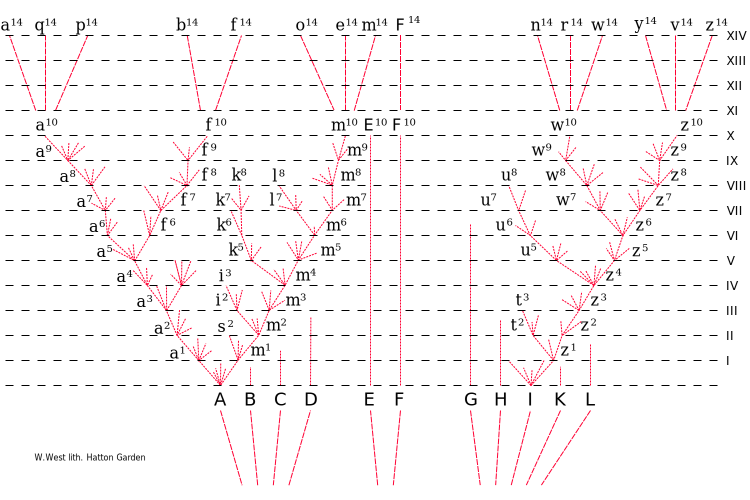
\includegraphics[width=0.90\textwidth]{introduction/darwin-tree.png}
    \caption{Darwin's abstract tree diagram illustrating evolutionary divergence over time. Modified from \textit{Inductiveload, Wikimedia Commons}.}
    \label{fig::intro::darwin-tree}
\end{figure}

\subsection{What Is a Phylogenetic Tree?}

A phylogenetic tree, or phylogeny, is a branching diagram that represents hypothesized evolutionary relationships among biological entities (e.g.\ species, populations, or genes) based on similarities and differences in their traits or genetic compositions. A typical phylogeny contains the following elements:
\begin{fancyenumerate}
    \item! \textbf{Root}: The most recent common ancestor of all entities represented in the tree.
    \item! \textbf{Branches}: Line segments representing evolutionary lineages.
    \item! \textbf{Nodes}: Points where branches join or split, typically interpreted as speciation or divergence events.
    \item! \textbf{Tips}: Terminal nodes representing the sampled taxa (extant or extinct) included in the analysis.
\end{fancyenumerate}

Trees can be \emph{rooted}, indicating a direction of time from the root to the tips, or \emph{unrooted}, which depict relationships among taxa without specifying an ancestral root. Mathematically, a phylogeny is a special case of a graph. Its topology can be rearranged visually---for example, by rotating subtrees around internal nodes or changing layout (rectangular, radial, unrooted)---without altering the underlying relationships, as long as connections among nodes are preserved (see \autoref{fig::intro::phylo-shapes}). For purely topological trees (those without meaningful branch lengths), even stretching or compressing branches does not affect the encoded relationships.

\begin{figure}[ht]
    \centering
    \resizebox{0.5\textwidth}{!}{
        \includesvg{introduction/phylo-shapes.svg}
    }
    \caption{Different layouts of the same phylogenetic tree. The blue circle marks the root, orange circles indicate internal nodes, and green circles indicate tips. Rearranging branches without changing their connections preserves the underlying topology.}
    \label{fig::intro::phylo-shapes}
\end{figure}

While phylogenies may include \emph{polytomies} (nodes with more than two descendants), they are often depicted as fully bifurcating trees. In many cases, multifurcations are treated as temporary placeholders for uncertainty that could be resolved into a series of bifurcations with additional data. Importantly, standard phylogenies are spatially implicit: they do not encode explicit geographic locations or distances.

Historically, researchers assembled phylogenies manually from morphological and anatomical comparisons. Today, phylogenies are inferred from biological data using computational methods, and they serve as the backbone for a wide variety of downstream analyses. In many molecular phylogenetic applications, trees reconstructed from extant data are treated as \emph{ultrametric}: all tips terminate at the same distance from the root and correspond to lineages observed at the present. This assumption underlies many phylogenetic algorithms and statistics.

\subsection{From Morphology and Similarity to Molecular Phylogenies}

Early phylogenetic inference relied heavily on morphology and anatomy. Researchers examined structural features of organisms to identify \emph{homologous} traits---characters inherited from a common ancestor \citep{haeckel_generelle_1866}. For example, the presence of four limbs in tetrapods is a classic homologous character. Shared homologous traits can be used to construct trees illustrating evolutionary relationships among groups (e.g.\ tetrapods in \autoref{fig::intro::homology-tree}). A major challenge in such analyses is distinguishing homologous traits from \emph{analogous} traits that evolved independently (e.g.\ wings in birds and insects), a distinction critical for accurate phylogenetic reconstruction \citep{irisarri_phylotranscriptomic_2017}.

\begin{figure}[ht]
    \centering
    \includegraphics[width=0.6\textwidth]{introduction/homology-tree.png}
    \caption{Example tree based on homologous characters (the presence of four limbs) in tetrapods. Recreated from \citet{irisarri_phylotranscriptomic_2017}.}
    \label{fig::intro::homology-tree}
\end{figure}

Phenetics, or numerical taxonomy, later emerged as a method for classifying organisms by overall similarity, often using quantitative measurements across many traits \citep{sokal_principles_1963}. The goal was to achieve objectivity by applying statistical methods to multivariate datasets, while avoiding explicit assumptions about evolutionary history. However, phenetic approaches were criticized for sometimes grouping taxa based on superficial similarity arising from convergent evolution, rather than true common ancestry \citep{de_queiroz_phenetic_1997}. Some taxonomists hoped that analyzing a sufficiently large number of characters would better cluster taxa descended from the nearest common ancestor, but this proved impractical: assembling and scoring many reliable characters was labor-intensive, and there is little guidance on which clustering or distance measures were appropriate in different situations \citep{mayr_taxonomy_2001,harvey_phylogeny_2001}.

The advent of large-scale DNA sequencing transformed phylogenetics. Molecular data allow researchers to compare DNA or protein sequences across a wide variety of organisms and to infer trees that depict their evolutionary relationships (see \autoref{fig::intro::modern-tree} for an example). These molecular phylogenies often corroborate traditional, morphology-based classifications but, in some cases, have prompted major revisions where genetic evidence reveals previously unrecognized relationships \citep{woese_towards_1990,cooper_quantitative_2003}. Fossil records play a complementary role: they provide temporal context, document extinct lineages, and offer morphological information not accessible from living taxa alone. Integrating fossil data with molecular trees enables calibration of molecular clocks and estimation of divergence times \citep{slater_integrating_2012,slater_unifying_2013,parham_best_2012}. Despite these advances, reconciling molecular and fossil evidence remains challenging due to incomplete fossil records \citep{wiens_missing_2003}, limitations on DNA preservation in ancient specimens \citep{yang_ancient_1997}, and complications from processes such as horizontal gene transfer \citep{moore_convergent_1997,kurland_horizontal_2003} and convergent evolution \citep{speed_quantification_2017,galtier_model_2007}.

\begin{figure}[ht]
    \centering
    \includegraphics[width=0.95\textwidth]{introduction/modern-tree.png}
    \caption{Example of a modern phylogeny based on DNA sequence data. Recreated from a \texttt{ggtree} illustration.}
    \label{fig::intro::modern-tree}
\end{figure}

\subsection{Alternative Tree Forms}

The classical phylogenetic tree is often presented as a strictly bifurcating hierarchy where all sampled taxa are tips, ancestors are unsampled, and evolution proceeds exclusively via splitting. In practice, several extensions of this basic model are widely used to capture more nuanced evolutionary scenarios. These include, for example, sampled ancestors \citep{morlon_reconciling_2011, slater_unifying_2013, heath_fossilized_2014, gavryushkina_bayesian_2014}, anagenesis \citep{wagner_probabilistic_2010, marshall_using_2019}, and polytomies \citep{maddison_reconstructing_1989, purvis_polytomies_1993, page_molecular_2009, drummond_bayesian_2015}.

Phylogenies can explicitly incorporate fossil taxa, often scored for morphological characters, alongside extant species. Rather than using fossils only as node calibrations, \emph{tip-dating} and \emph{total-evidence} approaches treat fossil species as tips with known ages and integrate them into the branching process \citep{slater_integrating_2012,parham_best_2012}. In these frameworks, both morphological and molecular characters contribute to the inference of topology and divergence times, and fossils may act as sampled ancestors. Including fossil taxa can break up long branches, reveal stem lineages leading to modern clades, and substantially alter interpretations of trait evolution and biogeography \citep{morlon_reconciling_2011,wiens_missing_2003}. Trees that integrate fossils in this way provide a more explicit, time-aware view of macroevolutionary history.

\subsection{Branch Lengths, Molecular Clocks, and Tree Types}

Before interpreting phylogenetic tree properties or attempting to extract quantitative information from a tree, it is essential to understand what branch lengths represent in a given case. Three broad categories are commonly distinguished (see \autoref{fig::intro::types-branch-length}):

\begin{fancyenumerate}
    \item! \textbf{Cladogram}: branch lengths carry no quantitative meaning; only the branching order matters.
    \item! \textbf{Phylogram}: branch lengths are proportional to the amount of genetic change (e.g.\ expected substitutions per site).
    \item! \textbf{Chronogram}: branch lengths are proportional to time, so that the path length from root to a tip reflects elapsed evolutionary time.
\end{fancyenumerate}

\begin{figure}[ht]
    \centering
    \includegraphics[width=0.95\textwidth]{introduction/types-branch-length.png}
    \caption{Three types of trees with different interpretations of branch length, adapted from Kellis \textit{et al.} \citep{kellis_computational_2020}. \textbf{Left:} a cladogram with no meaningful branch lengths. \textbf{Middle:} a phylogram in which branch lengths represent genetic change since divergence. \textbf{Right:} a chronogram (ultrametric tree) in which branch lengths represent time since divergence. All three trees share identical topology.}
    \label{fig::intro::types-branch-length}
\end{figure}

The classical molecular clock hypothesis assumes that genetic change accumulates at a roughly constant rate, so that branch lengths in a phylogram are proportional to divergence times when appropriately scaled \citep{robinson_molecular_2001}. Empirical studies, however, show that rates vary widely across lineages. Factors such as metabolic rate \citep{gillooly_metabolic_2004}, generation time \citep{fu_estimating_2001}, and environmental conditions \citep{bromham_exploring_2015,liu_yeast_2019} all influence substitution rates. Applying a single, global clock across distantly related taxa can therefore lead to inaccurate divergence time estimates.

To accommodate rate variation, a range of \emph{local}, \emph{discrete}, and \emph{relaxed} clock models have been developed. These allow rates to differ among branches or among clades while still linking molecular change to time \citep{lepage_general_2007,baele_accurate_2013,ho_molecular-clock_2014}. More flexible ``mixed'' branch-length models also allow for site-specific rate variation across the genome, improving both phylogeny inference and divergence-time estimation \citep{kolaczkowski_mixed_2008}. When comparing phylogenetic metrics across trees, it is crucial to account for these differences: the same statistic may have different interpretations on a cladogram, a phylogram, or a chronogram.

\subsection{What We Can Learn from Phylogenies}

Many of the hardest questions in evolution are hard because the past is unobserved: we do not directly see historical speciation, extinction, or the tempo of trait change. For many clades (especially those lacking a rich fossil record), the most information-rich record we often have is a phylogeny of extant taxa, which encodes both branching order and the timing of divergences. For example, when a novel pathogen spreads, time-calibrated phylogenies built from genome sequences can be used to reconstruct introductions, identify transmission clusters, and estimate how rapidly an epidemic is growing \citep{grenfell_unifying_2004,pybus_evolutionary_2009,stadler_birthdeath_2013}. In conservation, tree-based measures such as phylogenetic diversity and evolutionary distinctiveness help prioritize areas or lineages that represent disproportionate amounts of unique evolutionary history \citep{faith_conservation_1992,isaac_mammals_2007}. In community ecology and invasion biology, the phylogenetic structure of assemblages (clustering vs.\ overdispersion) is often used as a proxy for shared traits and niche similarity, informing hypotheses about environmental filtering, competition, and biotic resistance \citep{webb_exploring_2000,webb_phylogenies_2002,strauss_exotic_2006}.

These examples share a common logic: branching patterns summarize shared ancestry, while branch lengths carry information about the timing (or amount) of change. Phylogenies are therefore not merely static pictures of history; they are quantitative objects from which we can extract information about trait evolution, diversification dynamics, and community structure. Two broad classes of tools are especially important: phylogenetic comparative methods and tree summary statistics.

\subsubsection{Phylogenetic Comparative Methods}

Phylogenetic comparative methods use the shared evolutionary history encoded in a tree to test hypotheses about trait evolution while accounting for the non-independence of species. A foundational contribution is Felsenstein’s method of \emph{phylogenetically independent contrasts}, which transforms trait data on a tree into a set of contrasts that are statistically independent under a Brownian-motion model \citep{felsenstein_phylogenies_1985}. These contrasts can then be analyzed using standard regression or correlation techniques, while controlling for phylogenetic relatedness \citep{stadler_decoding_2024}.

Generalized least squares and related approaches extend this framework by explicitly modeling the covariance structure among species as a function of the tree and an evolutionary model \citep{rzhetsky_statistical_1992,symonds_primer_2014}. This allows hypothesis testing about processes such as adaptive evolution, constraint, or niche conservatism. Recent developments have pushed comparative methods into the high-dimensional regime. Penalized likelihood and Bayesian frameworks can accommodate many traits simultaneously and regularize complex models, enabling studies of multivariate trait evolution \citep{clavel_penalized_2019,adams_multivariate_2018,fuentes-g_bayesian_2020}.

\subsubsection{Tree Summary Statistics}

A large family of summary statistics has been proposed to quantify different aspects of tree shape, size, and timing (see \citep{janzen_phylogenetic_2024} for an overview). Although this thesis will discuss model-specific statistics later, it is useful here to highlight four broad classes:

\begin{fancyenumerate}
    \item! \textbf{Tree balance metrics}: These quantify how evenly lineages branch across the tree. Classical examples include the Sackin index, which sums the depths of all tips \citep{sackin_good_1972}, and Colless-type indices of imbalance \citep{janzen_phylogenetic_2024}. Imbalanced trees (with many short branches on one side of a split and long branches on the other) may indicate heterogeneous diversification rates or adaptive radiations.
    \item! \textbf{Branching-time statistics}: These describe the temporal pattern of divergence events. The gamma statistic, for instance, summarizes whether branching events are concentrated early or late relative to a constant-rate birth--death model \citep{pybus_testing_2000}. Deviations from the null expectation can suggest changes in diversification rates through time.
    \item! \textbf{Tree size and depth}: Simple metrics such as the number of tips (species richness) and tree height (the distance from root to most distant tip) provide basic information about the scale of the clade and the time available for diversification.
    \item! \textbf{Spectral and graph-theoretic metrics}: These approaches treat the phylogeny as a graph and summarize its structure via the eigenvalues of matrices such as the (distance) Laplacian or normalized Laplacian. The resulting spectral density profiles and derived statistics capture global features of connectivity and branching that are only partly reflected in classical imbalance or gamma-type metrics \citep{lewitus_characterizing_2016,chindelevitch_network_2021,janzen_phylogenetic_2024}.
\end{fancyenumerate}

The interpretation of these statistics depends strongly on what branch lengths represent (cladogram vs.\ phylogram vs.\ chronogram) and on how the tree was reconstructed. For example, comparing a gamma statistic or a Laplacian spectrum across trees inferred under different clock models or with different fossil calibrations can confound biology with methodology: apparent differences may simply reflect rescaled or redistributed branch lengths.

\subsection{Beyond Trees: Phylogenetic Networks}

The tree model implicitly assumes that lineages only split and never rejoin. However, many evolutionary processes violate this assumption. \emph{Reticulate} processes such as hybridization, introgression, horizontal gene transfer, and recombination create histories in which lineages merge as well as split (\autoref{fig::intro::tree-vs-network}). In such cases, representing evolution as a single bifurcating tree can be misleading: different genes may have different genealogies, and no single tree can capture all the relevant relationships \citep{moore_convergent_1997,kurland_horizontal_2003,huson_application_2006,galtier_model_2007}.

\begin{figure}[ht]
  \centering
  \begin{tikzpicture}[
    node distance=0.75cm,
    tip/.style={anchor=west},
    >=Stealth
  ]

  % Left panel: Tree
  \node[rug-red,font=\sffamily\bfseries\footnotesize,anchor=west] (labTree) at (-0.4,2.6) {Tree};

  % Backbone
  \coordinate (r1) at (0,2);
  \coordinate (a1) at (0.8,2);
  \coordinate (b1) at (0.8,1.2);
  \coordinate (c1) at (0.8,0.4);

  \coordinate (a1tip) at (2.2,2.4);
  \coordinate (b1tip) at (2.2,1.2);
  \coordinate (c1tip) at (2.2,0.0);

  \draw[treegray,thick]
    (r1) -- ++(-0.5,0)  % root stem
    (r1) -- (a1)
    (r1) -- (b1)
    (b1) -- (c1);

  \draw[treegray,thick]
    (a1) -- (a1tip)
    (b1) -- (b1tip)
    (c1) -- (c1tip);

  \node[tip,accentred] at (a1tip) {species A};
  \node[tip,accentred] at (b1tip) {species B};
  \node[tip,accentred] at (c1tip) {species C};

  % Axis arrow
  \draw[treegray,->,line width=0.4pt, yshift=-5] (-0.5,-0.2) -- (2.4,-0.2);
  \node[treegray,anchor=north,font=\sffamily\scriptsize, yshift=-5] at (1.0,-0.2)
    {divergence (tree-like)};

  % Right panel: Network
  \begin{scope}[xshift=6.0cm]
    \node[rug-red,font=\sffamily\bfseries\footnotesize,anchor=west] (labNet) at (-0.4,2.6) {Network};

    % Backbone tree
    \coordinate (r2) at (0,2);
    \coordinate (a2) at (0.8,2);
    \coordinate (b2) at (0.8,1.2);
    \coordinate (c2) at (0.8,0.4);

    \coordinate (a2tip) at (2.2,2.4);
    \coordinate (b2tip) at (2.2,1.2);
    \coordinate (c2tip) at (2.2,0.0);

    \draw[treegray,thick]
      (r2) -- ++(-0.5,0)
      (r2) -- (a2)
      (r2) -- (b2)
      (b2) -- (c2);

    \draw[treegray,thick]
      (a2) -- (a2tip)
      (b2) -- (b2tip)
      (c2) -- (c2tip);

    % Reticulation edge from A lineage into C lineage
    \draw[dashed,accentorange,thick,->]
      (1.4,2.2) .. controls (1.8,1.9) and (1.8,0.8) .. (1.4,0.4);

    % Tips
    \node[tip,accentred] at (a2tip) {species A};
    \node[tip,accentred] at (b2tip) {species B};
    \node[tip,accentred] at (c2tip) {species C};

    \node[accentorange,anchor=west,font=\sffamily\scriptsize, yshift=15] at (1.9,1.2)
      {gene flow / hybridization};
  \end{scope}

  \end{tikzpicture}
  \caption{From a strictly bifurcating tree (\textbf{left}) to a simple phylogenetic network (\textbf{right}) with a reticulation event connecting two lineages.}
  \label{fig::intro::tree-vs-network}
\end{figure}


Phylogenetic networks generalize trees by allowing edges that represent reticulation events \citep{huson_application_2006}. Conceptually, a phylogenetic network is a graph in which some nodes may have more than one parent, corresponding, for example, to a hybrid species with two ancestral lineages or to a genome that has acquired genes by lateral transfer. Several types of networks are commonly distinguished:

\begin{fancyenumerate}
    \item! \textbf{Implicit (split) networks}: These networks, such as neighbor-net or related methods, are largely exploratory. They visualize conflicting phylogenetic signals as cycles or boxes, without requiring that internal nodes correspond to actual ancestral taxa (\autoref{fig::intro::split-net}). Such networks are useful for highlighting data conflict or potential reticulation \citep{bryant_neighbor-net_2004, huson_application_2006}.
    \item! \textbf{Explicit (hybridization or species) networks}: These represent hypothesized evolutionary histories where some internal nodes are hybrids or result from gene flow between lineages \citep{warnow_advances_2019, solis-lemus_phylonetworks_2017, hibbins_phylogenomic_2022}. Here, nodes often have a direct biological interpretation, and reticulation edges correspond to specific evolutionary events (e.g.\ hybrid speciation in plants or introgression among closely related animals).
    \item! \textbf{Ancestral recombination graphs (ARGs)}: Widely used in population genetics, ARGs describe the genealogy of genetic segments in a recombining population. Recombination events introduce reticulation so that different parts of a genome trace back through different ancestral paths \citep{griffiths_ancestral_1997, lewanski_era_2024}.
\end{fancyenumerate}

\begin{figure}[ht]
  \centering
  \begin{tikzpicture}[
    node distance=1.4cm,
    tip/.style={circle,inner sep=1pt},
    >=Stealth
  ]

  % Background highlight for conflicting area
  \fill[pastelpink] (0.4,0.0) -- (3.0,0.0) -- (3.0,2.0) -- (0.4,2.0) -- cycle;

  % Nodes
  \node[tip] (A) at (0,1.5) {};
  \node[tip] (B) at (0,0.5) {};
  \node[tip] (C) at (3.4,1.5) {};
  \node[tip] (D) at (3.4,0.5) {};

  % Labels
  \node[accentred,anchor=east] at (A.west) {taxon A};
  \node[accentred,anchor=east] at (B.west) {taxon B};
  \node[accentred,anchor=west] at (C.east) {taxon C};
  \node[accentred,anchor=west] at (D.east) {taxon D};

  % Internal junctions for two alternative splits
  \coordinate (L1) at (0.8,1.0);
  \coordinate (R1) at (2.6,1.0);
  \coordinate (L2) at (0.8,1.8);
  \coordinate (R2) at (2.6,0.2);

  % Split 1: (A,B)|(C,D)
  \draw[treegray,thick]
    (A) -- (L1)
    (B) -- (L1)
    (C) -- (R1)
    (D) -- (R1)
    (L1) -- (R1);

  % Split 2: (A,D)|(B,C) forming the box
  \draw[accentorange,thick,dashed]
    (A) -- (L2) -- (R2) -- (D) -- cycle;

  % Annotation
  \node[rug-red,anchor=south west,font=\sffamily\footnotesize] at (0.5,2.05)
    {Conflicting splits};
  \node[treegray,anchor=north,font=\sffamily\scriptsize] at (1.7,-0.2)
    {split network (data conflict as boxes)};

  \end{tikzpicture}
  \caption{Toy split network for four taxa. Two incompatible splits form a ``box'', illustrating conflicting phylogenetic signal that cannot be represented on a single bifurcating tree.}
  \label{fig::intro::split-net}
\end{figure}


Reticulate evolution is especially prominent in microbes, where horizontal gene transfer can blur species boundaries and produce a ``web of life'' rather than a simple tree \citep{moore_convergent_1997,doolittle_phylogenetic_1999,kurland_horizontal_2003, bapteste_networks_2013}. In plants, hybridization and polyploidization are frequent and can drive rapid diversification \citep{linder_reconstructing_2004, marhold_polyploidy_2006}. Even in animals, genome-scale data have revealed pervasive introgression events (e.g.\ among hominins), challenging purely tree-like views of evolution \citep{racimo_evidence_2015,martin_interpreting_2017}. In all of these cases, networks provide a potentially more faithful qualitative model of evolutionary history than trees alone.

At the same time, networks are more complex to infer and interpret than trees, and the data requirements for confidently identifying reticulation events are substantial \citep{huson_application_2006}. For many questions, a tree remains an adequate and more parsimonious representation. A practical strategy is therefore to treat phylogenetic trees as a baseline model and to invoke network representations when there is clear evidence that simple branching is insufficient \citep{warnow_advances_2019, hibbins_phylogenomic_2022}. In this thesis, the focus will be on \emph{trees with calendar time units (chronograms)} and \emph{tree-based statistics}, while keeping in mind that many real evolutionary histories are embedded in richer, network-like structures. 

\clearpage
\section{Phylogenetic Birth--Death Models}
\dropcap{P}hylogenetic birth--death models provide a simple but powerful probabilistic framework for describing how speciation (``birth'') and extinction (``death'') events generate branching trees through time. In the classical constant-rate model, each lineage gives rise to new species at rate $\lambda$ and goes extinct at rate $\mu$, independently of other lineages and of time \citep{nee_extinction_1994,nee_reconstructed_1994,nee_birth-death_2006}. When $\lambda>\mu$, the expected number of lineages grows approximately exponentially, and in the absence of extinction ($\mu=0$) the process reduces to a pure-birth Yule model. Because empirical phylogenies often include only extant species, we typically observe a \emph{reconstructed} tree, in which extinct lineages have been pruned away. For such reconstructed trees, constant-rate birth--death theory predicts that lineage-through-time (LTT) plots---tracking the number of lineages with descendants at the present---should exhibit a characteristic upturn near the present, often called the ``pull of the present'', as illustrated in the left panel of \autoref{fig::intro::ltt} \citep{kubo_inferring_1995,nee_extinction_1994,stadler_decoding_2024}. Intuitively, this arises because lineages that survive to the present have not had enough time to go extinct, so the observed extinction rate near the present is reduced and net diversification appears to accelerate \citep{etienne_diversity-dependence_2012}.

\begin{figure}[ht]
  \centering
  \begin{tikzpicture}[
    >=Stealth,
    x=1cm,
    y=1cm
  ]

  % Left panel: constant-rate BD with extinction
  \begin{scope}
    % axes
    \draw[treegray,->] (0,0) -- (4,0) node[anchor=west] {\scriptsize time};
    \draw[treegray,->] (0,0) -- (0,3) node[anchor=south] {\scriptsize $\log$(lineages)};

    % log N(t) = a + r0 * t + b * t^3
    \draw[accentorange,thick,smooth,domain=0.2:3.5,samples=200]
      plot (\x,{0.6 + 0.15*\x + 0.018*pow(\x,3)});

    % label
    \node[gray,anchor=west,yshift=4] at (1.0,2.0)
      {\scriptsize constant-rate BD with extinction};
    \node[rug-red,font=\sffamily\bfseries\footnotesize,anchor=west,yshift=15] at (0,3.15)
      {Pull of the present};
  \end{scope}

  % Right panel: diversity-dependent BD (logistic N(t)) on log scale
  \begin{scope}[xshift=6cm]
    % axes
    \draw[treegray,->] (0,0) -- (4,0) node[anchor=west] {\scriptsize time};
    \draw[treegray,->] (0,0) -- (0,3) node[anchor=south] {\scriptsize $\log$(lineages)};

    % carrying capacity line
    \draw[treegray,dashed] (0.2,2.3) -- (3.8,2.3);
    \node[treegray,anchor=west] at (3.85,2.3) {\scriptsize $\log K$};

    % decelerating log-LTT
    \draw[accentred,thick,smooth,domain=0.2:3.5,samples=200]
      plot (\x,{2.3 - ln(1 + 7*exp(-1.0*\x))});

    % label
    \node[gray,anchor=west,yshift=-2] at (1.0,1.0)
      {\scriptsize diversity-dependent slowdown};

    \node[rug-red,font=\sffamily\bfseries\footnotesize,anchor=west,yshift=15] at (0,3.15)
      {Diversity-dependent birth--death};
  \end{scope}

  \end{tikzpicture}
  \caption{Lineage-through-time (LTT) plots. \textbf{Left}: approximate expected log LTT under a constant-rate birth--death model with extinction, where the slope increases from the net diversification rate $\lambda-\mu$ early on toward the speciation rate $\lambda$ near the present, illustrating the pull of the present. \textbf{Right}: diversity-dependent model with carrying capacity $K$, where the expected log LTT (red) gradually approaches $\log K$ (dashed line) as diversification slows down.}
  \label{fig::intro::ltt}
\end{figure}


Nonetheless, many empirical phylogenies do not meet this simple expectation. Across a wide range of clades, LTT curves instead show a \emph{slowdown} in lineage accumulation toward the present: the log-lineage count bends downward rather than upward, suggesting that net diversification has decreased over time \citep{purvis_phylogenetic_2008,phillimore_density-dependent_2008,moen_why_2014,aguilee_clade_2018}. This pattern contrasts with what constant-rate models predict and also with some fossil-based reconstructions of diversity, which often show long-term saturation or fluctuating equilibria rather than recent slowdowns \citep{etienne_diversity-dependence_2012,louca_why_2021}. Reconciling these discrepancies has motivated a variety of extensions to the basic birth--death framework.

Several classes of mechanisms can generate decelerating LTT curves \citep{moen_why_2014,stadler_decoding_2024}:

\begin{fancyenumerate}
    \item! \textbf{Time-dependent diversification rates}: Speciation and/or extinction rates may change through time due to extrinsic factors (e.g.\ climatic shifts, geological events) or intrinsic evolutionary innovations. For instance, models in which speciation rates decline monotonically through time---sometimes interpreted as decreasing ecological opportunity---can produce early bursts of diversification followed by slowdowns \citep{moen_why_2014,morlon_reconciling_2011,stadler_inferring_2011}.
    \item! \textbf{Protracted speciation}: Under protracted birth--death models, speciation is treated as a multi-stage process rather than an instantaneous event. Lineages first enter an incipient-species state and only later complete speciation, or may fail to do so and be reabsorbed \citep{etienne_prolonging_2012,rosindell_protracted_2010}. Because recently initiated speciation events are not yet counted as full species, protracted speciation reduces recent apparent diversification and counteracts the pull of the present. This process is illustrated in \autoref{fig::intro::protracted-bd}.
    \item! \textbf{Negative diversity-dependent diversification}: In diversity-dependent diversification (DDD) models, speciation rates decrease (and/or extinction rates increase) as the number of species in a clade rises. This can reflect competition for finite resources or niche space, leading to an effective carrying capacity $K$ for diversity \citep{valentine_evolutionary_1974,sepkoski_kinetic_1978,etienne_diversity-dependence_2012}. Early in a clade's history, when diversity is low, speciation proceeds nearly unhindered; as diversity approaches $K$, the net diversification rate declines and LTT curves tend to level off, as in the right panel of \autoref{fig::intro::ltt} \citep{wiens_causes_2011}.
    \item! \textbf{Incomplete and non-random sampling}: Empirical phylogenies often include only a fraction of the extant diversity \citep{pybus_testing_2000, cusimano_slowdowns_2010, hohna_inferring_2011}. Missing taxa---especially when sampling is biased toward deeper nodes and recent lineages are underrepresented---inflate terminal waiting times and can make lineage accumulation appear to slow toward the present even if diversification rates were constant \citep{cusimano_slowdowns_2010}. Interestingly, protracted speciation can be viewed as a related form of incomplete sampling: the underlying process contains incipient species, but the reconstructed tree records only completed species. Not all incipient lineages are ``observed'' as distinct taxa.
\end{fancyenumerate}

\begin{figure}[ht]
  \centering
  \begin{tikzpicture}[
    >=Stealth,
    x=0.8cm,
    y=0.8cm
  ]

  % Time axis
  \draw[treegray,->] (0,0) -- (10.5,0) node[anchor=west] {\scriptsize time};

  % Parent lineage
  \draw[treegray,thick] (1,1.0) -- (10.5,1.0);
  \node[treegray,anchor=east] at (1,1.0) {\scriptsize ancestral lineage};

  % Instantaneous speciation (reference)
  \draw[accentblue,thick] (1.4,1.0) -- (1.4,1.4);
  \draw[accentblue,thick] (1.4,1.4) -- (3.2,2.0);
  \node[accentblue,anchor=west] at (3.3,2.0) {\scriptsize instantaneous speciation};

  % Protracted speciation: incipient then good
  % Incipient branch
  \draw[accentorange,thick,dashed]
    (5.0,1.0) -- (5.7,1.4) node[pos=0.35,above right,xshift=-24] {\scriptsize incipient};
  % Transition to good species
  \draw[accentred,thick]
    (5.7,1.4) -- (7.5,2.0);
  \node[accentred,anchor=west] at (7.6,2.0) {\scriptsize completed speciation};

  % Protracted speciation: incipient then merge back
  % Incipient branch
  \draw[accentorange,thick,dashed]
    (8.0,1.0) -- (8.7,1.4) node[pos=0.35,above right,xshift=-24] {\scriptsize incipient};
  % Transition to good species
  \draw[treegray,thick,dashed]
    (8.7,1.4) -- (9.4,1.0);
    
  % Vertical markers for onset / completion
  \draw[treegray,dotted] (1.4,0) -- (1.4,1.0);
  \node[treegray,anchor=north,xshift=-10] at (1.4,0) {\scriptsize completion};
  \draw[treegray,dotted] (5.0,0) -- (5.0,1.0);
  \node[treegray,anchor=north,xshift=-4,yshift=-1] at (5.0,0) {\scriptsize onset};
  \draw[treegray,dotted] (5.7,0) -- (5.7,1.4);
  \node[treegray,anchor=north,xshift=10,yshift=-0.55] at (5.7,0) {\scriptsize completion};
  \draw[treegray,dotted] (8.0,0) -- (8.0,1.0);
  \node[treegray,anchor=north,yshift=-1] at (8.0,0) {\scriptsize onset};
  \draw[treegray,dotted] (9.4,0) -- (9.4,1.0);
  \node[treegray,anchor=north,yshift=-0.55] at (9.4,0) {\scriptsize merged};

  \end{tikzpicture}
  \caption{Illustration of protracted speciation. A new lineage enters an incipient-species stage (dashed orange) before becoming a fully recognized species (solid red), delaying the appearance of new species in reconstructed phylogenies relative to instantaneous speciation. A new lineage may fail and merge back.}
  \label{fig::intro::protracted-bd}
\end{figure}


In negative diversity-dependent models, species richness is usually treated as a single scalar state variable that summarizes competition, niche occupancy, and other ecological interactions. In practice, species act as proxies for mechanistic factors such as functional traits, ecological niches, and biotic interactions that ultimately shape ecological limits \citep{srivastava_phylogenetic_2012,kondratyeva_reconciling_2019}. This implicitly assumes that all species contribute equally to filling ecological space.

\begin{figure}[ht]
  \centering
  \begin{tikzpicture}[
    x=0.6cm,
    y=0.6cm,
    >=Stealth
  ]

  % --- Left: equivalent species ---
  \begin{scope}
    % big niche box
    \draw[accentred,dashed,thick,rounded corners]
      (0,0) rectangle (5.17,3);
    \node[accentred,anchor=south west] at (0,3.05)
      {\scriptsize total niche space};

    % identical species boxes
    \foreach \x/\y in {0.3/0.3, 1.5/0.3, 2.7/0.3, 3.9/0.3,
                       0.3/1.2, 1.5/1.2, 2.7/1.2, 3.9/1.2,
                       0.3/2.1, 1.5/2.1, 2.7/2.1, 3.9/2.1} {
      \draw[treegray,fill=pastelblue] (\x,\y) rectangle ++(1.0,0.6);
    }

    \node[treegray,anchor=north west] at (0, -0.3)
      {\scriptsize species treated as equivalent};
  \end{scope}

  % --- Right: relatedness-dependent niches ---
  \begin{scope}[xshift=4.2cm]
    % big niche box
    \draw[accentred,dashed,thick,rounded corners]
      (0,0) rectangle (5.17,3);
    \node[accentred,anchor=south west] at (0,3.05)
      {\scriptsize total niche space};

    % species with varying widths & colors
    % clade 1 (similar, close relatives)
    \draw[fill=pastelblue,draw=treegray] (0.3,0.3) rectangle ++(1.4,0.6);
    \draw[fill=pastelblue!80!accentred,draw=treegray] (1.8,0.3) rectangle ++(1.3,0.6);
    \draw[fill=pastelblue!60!accentred,draw=treegray] (3.2,0.3) rectangle ++(1.1,0.6);

    % clade 2 (different niche cluster)
    \draw[fill=pastelpink,draw=treegray] (0.4,1.4) rectangle ++(0.9,0.7);
    \draw[fill=pastelpink!90!accentorange,draw=treegray] (1.6,1.5) rectangle ++(1.6,0.6);

    % a highly distinct species
    \draw[fill=accentorange!40,draw=treegray,thick] (3.0,2.0) rectangle ++(1.8,0.8);

    % little tombstones for extinctions
    \draw[treegray,fill=treegray!10] (0.6,2.1) -- ++(0.0,0.4) -- ++(0.3,0) -- ++(0,-0.4) -- cycle;
    \draw[treegray,fill=treegray!10] (2.3,0.9) -- ++(0.0,0.4) -- ++(0.3,0) -- ++(0,-0.4) -- cycle;

    \node[treegray,anchor=north west, xshift=-5.4] at (0, -0.3)
      {\scriptsize niches structured by relatedness};
  \end{scope}

  \end{tikzpicture}
  \caption{Conceptual illustration of species non-equivalence. Left: all species are treated as equivalent units occupying similar amounts of niche space. Right: niche widths and positions differ, reflecting evolutionary relatedness and ecological similarity; closely related species cluster in niche space and may interact more strongly.}
  \label{fig::intro::niche-space-tile}
\end{figure}


Yet species may not be equivalent entities, as illustrated in \autoref{fig::intro::niche-space-tile}. Closely related species tend to share similar traits and ecological requirements due to common ancestry; they may compete more strongly, respond similarly to environmental change, or share enemies \citep{srivastava_phylogenetic_2012,helmus_phylogenetic_2007,cadotte_phylogenetic_2012,pigot_quantifying_2016}. Phylogenetic or evolutionary relatedness thus provides a convenient proxy for ecological similarity and potential interaction strength. For example, in invasion biology, species that are evolutionarily distant from the resident community can be more successful colonists, presumably because they occupy distinct niches and face less competition from close relatives \citep{zheng_species_2018,henn_environmental_2019,qin_phylogenetic_2020}. 

However, being \emph{too} distantly related may also imply a poor match to the local abiotic environment, so that environmental filtering prevents establishment even if competition is weak. This tension between reduced biotic resistance and reduced abiotic fit is one facet of Darwin’s naturalization “conundrum” and indicates that performance may peak at intermediate relatedness rather than changing monotonically \citep{gallien_contrasting_2015, ma_different_2016, park_darwins_2020}. Taken together, the impact of an additional species on diversification dynamics is very likely to hinge on \emph{how closely related} it is to other members of the clade, a concept illustrated in \autoref{fig::intro::niche-space}.

\begin{figure}[ht]
    \centering
    \includegraphics[width=0.85\textwidth]{introduction/niche-space.png}
    \caption{Species may not be equivalent entities; their traits and niche spaces can be influenced by their evolutionary relatedness. The left panel illustrates a scenario where all species are considered equivalent, with no regard for relatedness. In contrast, the right panel depicts a scenario where evolutionary relatedness affects traits and niche spaces. The phylogenetic trees in both panels are identical. Tombstone signs mark species that have gone extinct. The red dashed boxes represent the total hypothetical niche space, while the smaller colored boxes indicate the niche spaces occupied by individual species. The color gradient of these smaller boxes reflects the degree of similarity between species, and their width represents the amount of niche space each species occupies.}
    \label{fig::intro::niche-space}
\end{figure}

Most empirical and theoretical work on diversity-dependent diversification has focused on single clades and has assumed that all species within the focal clade contribute equally to limiting diversity \citep{rabosky_equilibrium_2010,etienne_diversity-dependence_2012,foote_diversity-dependent_2018}. Fewer studies have explored cross-clade or cross-lineage interactions, or explicitly distinguished between the effects of close vs.\ distant relatives \citep{pires_interactions_2017}. A recent island-frog study \citep{etienne_phylogenetic_2023} showed that diversity-dependence among closely related species had much stronger effects on colonization and diversification than interactions with more distantly related species, underscoring the importance of phylogenetic scale.

To date, few birth--death models have made evolutionary relatedness an explicit determinant of diversification rates. A natural next step is to use \emph{phylogenetic metrics} based on branch lengths---such as pairwise distances or measures of evolutionary distinctiveness---to modulate speciation and extinction rates in simulations. This is particularly appealing because most birth--death simulation algorithms produce chronograms (branch lengths proportional to time), so time since divergence is directly available and can be interpreted as a proxy for accumulated genetic and ecological differences. 

At the same time, birth--death theory reveals that the distribution of branch lengths in simulated trees can be unintuitive. For example, under a pure-birth Yule process, the expected lengths of internal and pendant branches are surprisingly similar and on average shorter than might be naively expected \citep{mooers_branch_2012}. Because many inference methods are sensitive to branch length distributions, it is crucial to be explicit about what branch lengths represent (time, amount of genetic change, or arbitrary units, as we discussed before) and how they were estimated \citep{nee_birth-death_2006,etienne_diversity-dependence_2012}. When we tie diversification rates to branch-length-based metrics, we implicitly assume that divergence time is a reasonable proxy for the accumulation of genetic and ecological differences. This assumption may hold in some systems but not in others. 

Overall, birth--death models have evolved from simple constant-rate descriptions to increasingly rich frameworks that incorporate time-dependence, diversity-dependence, protracted speciation and many more \citep{maddison_estimating_2007,fitzjohn_diversitree_2012,valente_equilibrium_2015,caetano_hidden_2018, herrera-alsina_detecting_2019}. In this thesis, we will introduce a new extension that incorporates dependence on \emph{both diversity and evolutionary relatedness}. Together, these models provide a conceptual bridge between individual-level evolutionary or ecological processes and the large-scale patterns observed in phylogenies and the fossil record. To assess their adequacy and to infer their parameters from data, we rely on a suite of statistical tools, which we discuss next.

\clearpage
\section{Inference of Diversification from Phylogenies}
\dropcap{I}nference tools play a central role in connecting birth--death models to empirical data. Given a reconstructed, time-calibrated phylogeny and, where available, fossil information, our goal is to infer diversification parameters (e.g.\ speciation and extinction rates) and to assess whether patterns such as time-dependence, diversity-dependence, or trait-dependence are supported. Time-calibrated phylogenies encode both branching times and topological relationships among species and thus provide a complementary source of information to the often incomplete fossil record \citep{kidwell_quality_1996}. When the assumed birth--death model approximates the true underlying process, it is possible to estimate speciation and extinction rates from such trees \citep{nee_reconstructed_1994,nee_inferring_2001,morlon_phylogenetic_2014}. 

\subsection{Likelihood-Based/Bayesian Methods}
Classical approaches to diversification inference rely on \emph{likelihood}-based frameworks. For a given birth--death model and parameter values, one can, in many cases, write down the probability of observing a particular reconstructed tree (or at least its ranked branching times) under that model \citep{nee_extinction_1994,nee_reconstructed_1994,stadler_simulating_2011,stadler_decoding_2024}. Maximizing this likelihood over the parameter space yields maximum likelihood estimates (MLEs) of speciation and extinction rates \citep{morlon_phylogenetic_2014,etienne_how_2016}; alternatively, embedding the likelihood in a Bayesian framework allows one to obtain posterior distributions for parameters via Markov chain Monte Carlo (MCMC) sampling \citep{xie_identifying_2023}. 

Over the past two decades, likelihood-based models have been extended in several directions. Time-varying models allow speciation and extinction rates to change as functions of time or environmental covariates \citep{morlon_reconciling_2011,stadler_inferring_2011}. Diversity-dependent models explicitly link rates to the current number of species in the clade \citep{etienne_diversity-dependence_2012,etienne_estimating_2014,valente_equilibrium_2015}. Trait-dependent or state-dependent models (e.g.\ BiSSE and its extensions) allow speciation and extinction to depend on discrete or continuous traits evolving along the tree \citep{maddison_estimating_2007,fitzjohn_diversitree_2012,alexander_quantifying_2016}. Likelihood-based methods for these models underpin many macroevolutionary analyses in the literature, and they remain the standard against which new approaches are often compared.

However, likelihood-based inference also faces important challenges. Closed-form likelihood expressions are only available for relatively simple models; more complex models can require intricate derivations or numerical approximations that are computationally expensive \citep{janzen_approximate_2015,lambert_deep_2023}. For many biologically realistic scenarios---for example, models with strong lineage heterogeneity or multiple interacting clades---deriving a tractable likelihood is prohibitively difficult. Even when a likelihood is available, identifiability issues can limit what can be learned from a single extant-only tree: different combinations of speciation and extinction rates may produce virtually indistinguishable reconstructed trees, especially when extinction is high \citep{rabosky_extinction_2010,louca_why_2021}. Small trees further exacerbate estimation bias; for example, MLEs of extinction often collapse to zero for modest-sized trees even when the true extinction rate is nonzero, whereas estimates improve as tree size (number of tips) increases \citep{etienne_how_2016}. Likelihood-based methods with many free parameters can also be prone to overfitting and may yield unstable estimates when data are limited \citep{ward_review_2008}.

\subsection{Approximate Bayesian Computation}
When likelihoods are unavailable or too costly to compute, \emph{Approximate Bayesian Computation} (ABC) offers an alternative route to parameter inference. ABC approximates the posterior distribution of parameters by (i) simulating data under proposed parameter values, (ii) summarizing both simulated and observed data by a set of summary statistics, and (iii) retaining parameter values that produce simulated statistics close to the observed ones \citep{beaumont_approximate_2002,beaumont_approximate_2010}. In principle, ABC can handle any diversification model so long as it is easy to simulate phylogenies from it.

In phylogenetics, however, applications of ABC remain relatively scarce \citep{rabosky_heritability_2009,bokma_time_2010,kutsukake_simulation-based_2013,xie_can_2023}. A central difficulty is choosing informative yet low-dimensional summary statistics that capture the relevant aspects of tree shape and branching times. Simple statistics, such as tree balance indices, the gamma statistic, or LTT-based features, may not be sufficient to distinguish between, say, time-dependent and diversity-dependent scenarios. In contrast, including many statistics can lead to a high-dimensional summary space in which ABC performs poorly. As a result, while ABC is conceptually attractive for complex birth--death models, careful design of summary statistics and distance metrics is critical and has so far limited its routine use in diversification studies \citep{xie_can_2023}.

\subsection{Machine Learning and Deep Learning Approaches}
Rapid advances in machine learning (ML)---particularly deep learning---offer new possibilities for inferring macroevolutionary parameters from phylogenetic data. Deep neural networks are function approximators that can learn complex, nonlinear relationships between inputs and outputs from large training datasets \citep{aggarwal_neural_2018}. \autoref{fig::intro::mlp} illustrates a simple example of a neural network architecture. In our context, the inputs are phylogenetic trees (or representations thereof), and the outputs are diversification parameters or model labels. Unlike classical ABC, deep learning can learn directly from high-dimensional or raw representations of trees without requiring hand-crafted summary statistics.

\begin{figure}[t]
  \centering
  \begin{tikzpicture}[
      >=stealth,
      node distance=1.2cm and 1.8cm,
      every node/.style={font=\small},
      neuron/.style={circle, draw, minimum size=10pt, inner sep=0pt},
      layerlabel/.style={font=\footnotesize\sffamily}
    ]

    % Input layer
    \foreach \i in {1,...,4} {
      \node[neuron, fill=gray!10] (I-\i) at (0, {-(\i-1)*1.0}) {};
    }
    \node[layerlabel, above=0.2cm of I-1, rug-red] {input layer};

    % Hidden layer
    \foreach \i in {1,...,5} {
      \node[neuron, fill=accentblue!10] (H-\i) at (2.3, {-(\i-1)*0.9+0.5}) {};
    }
    \node[layerlabel, above=0.2cm of H-1, rug-red] {hidden layer};

    % Output layer
    \foreach \i in {1,...,2} {
      \node[neuron, fill=red!10] (O-\i) at (4.6, {-(\i-1)*1.0-0.8}) {};
    }
    \node[layerlabel, above=0.2cm of O-1, rug-red] {output layer};

    % Connections: input to hidden
    \foreach \i in {1,...,4} {
      \foreach \j in {1,...,5} {
        \draw[->, thin] (I-\i) -- (H-\j);
      }
    }

    % Connections: hidden to output
    \foreach \i in {1,...,5} {
      \foreach \j in {1,...,2} {
        \draw[->, thin] (H-\i) -- (O-\j);
      }
    }

    % Labels for inputs/outputs
    \node[left=0.5cm of I-2] {$x_1,\dots,x_4$};
    \node[right=0.5cm of O-1] {$y_1,y_2$};

    % Legend arrow: gradient flow
    \begin{scope}[shift={(-0.2,-3.7)}]
      \draw[->, thin, gray] (1,0) -- (2,0);
      \node[font=\footnotesize, right=0.2cm] at (2,0)
        {information flow};
    \end{scope}
    
  \end{tikzpicture}
  \caption{Illustrative multi-layer perceptron with one hidden layer. Each neuron in a layer is fully connected to all neurons in the next layer, and information flows from left to right. This feed-forward architecture represents a basic building block of neural networks; deeper, convolutional, recurrent, or more complex models can all be viewed as extensions or refinements of this simple layered structure.}
  \label{fig::intro::mlp}
\end{figure}


A range of network architectures and tree representations has been explored:

\begin{fancyenumerate}
    \item! \textbf{Feature-based encodings and feed-forward networks}: One strategy is to compute vectors of tree-level features (e.g.\ branching-time summaries, balance indices, LTT-derived quantities) and feed them into standard multilayer perceptrons. This is straightforward to implement and has been used in several early applications of neural networks to phylogenetic data \citep{zhu_benchmarking_2018,lambert_deep_2023}. Its performance, however, depends heavily on the choice of features.
    \item! \textbf{Sequence encodings and recurrent neural networks}: Another approach is to serialize information about the tree, for example by ordering internal node ages from root to tips and treating the resulting sequence as a time series. Recurrent neural networks (RNNs), including LSTM and GRU variants, are designed to handle such sequential data and can therefore capture temporal dependencies in branching patterns \citep{sak_long_2014,salehinejad_recent_2017}. This allows them to learn from the ordered history of diversification events rather than from aggregated summaries.
    \item! \textbf{Graph-based representations and graph neural networks}: Because phylogenies are graph-structured, graph neural networks (GNNs) offer an attractive way to process them directly. In GNNs, each node (e.g.\ a speciation event or species) aggregates information from its neighbors over multiple message-passing layers, yielding a learned representation of the entire tree that can be used for parameter prediction \citep{kipf_semi-supervised_2016,ying_hierarchical_2018,li_deepergcn_2020,rampasek_recipe_2022, lajaaiti_comparison_2023}. This avoids discarding structural information but requires careful design of node and edge features.
    \item! \textbf{Topology-aware vectorizations and convolutional networks}: Recently, compact bijective encodings or ladderized vectorizations of trees have been proposed, which map each tree to a fixed-length vector or matrix encoding both topology and branch lengths. Convolutional neural networks (CNNs), originally developed for image recognition, can then be applied to these encodings to detect local patterns associated with particular parameter values \citep{voznica_deep_2022,lambert_deep_2023,lajaaiti_comparison_2023,moi_reconstructing_2022,reiman_popphy-cnn_2020}. These methods can automatically learn rich summary features without manual feature engineering.
\end{fancyenumerate}

Empirical evaluations of deep learning for diversification inference are encouraging. \citet{lambert_deep_2023} trained CNN-based models on simulated phylogenies under both homogeneous birth--death and state-dependent models and found that their networks could accurately recover speciation and extinction rates, often matching or exceeding the performance of MLE while being orders of magnitude faster at prediction. Similarly, \citet{voznica_deep_2022} and \citet{reiman_popphy-cnn_2020} demonstrated that deep learning models can infer epidemiological parameters from pathogen phylogenies. \citet{lajaaiti_comparison_2023} and \citet{qin_parameter_2025} compared multiple architectures (e.g. feed-forward, CNN, GNN) and highlighted trade-offs between flexibility, data requirements, and robustness across models.

\begin{figure}[t]
  \centering
  \begin{tikzpicture}[
      >=stealth,
      node distance=1.2cm and 1.8cm,
      every node/.style={font=\small},
      neuron/.style={circle, draw, minimum size=10pt, inner sep=0pt},
      layerlabel/.style={font=\footnotesize\sffamily}
    ]

    % Input layer
    \foreach \i in {1,...,4} {
      \node[neuron, fill=gray!10] (I-\i) at (0, {-(\i-1)*1.0}) {};
    }
    \node[layerlabel, above=0.2cm of I-1, rug-red] {input layer};

    % Hidden layer
    \foreach \i in {1,...,5} {
      \node[neuron, fill=accentblue!10] (H-\i) at (2.3, {-(\i-1)*0.9+0.5}) {};
    }
    \node[layerlabel, above=0.2cm of H-1, rug-red] {hidden layer};

    % Output layer
    \foreach \i in {1,...,2} {
      \node[neuron, fill=red!10] (O-\i) at (4.6, {-(\i-1)*1.0-0.8}) {};
    }
    \node[layerlabel, above=0.2cm of O-1, rug-red] {output layer};

    % Loss node on the right
    \node[draw, rounded corners, font=\footnotesize, color=accentorange!70]
      (Loss)
      at ($ (O-1)!0.5!(O-2) + (1.6cm,0) $)
      {$\mathcal{L}$};

    % Gradient flow: hidden to input
    \foreach \i in {1,...,4} {
      \foreach \j in {1,...,5} {
        \draw[<-, dashed, thin, gray] (I-\i) -- (H-\j);
      }
    }

    % Gradient flow: output to hidden
    \foreach \i in {1,...,5} {
      \foreach \j in {1,...,2} {
        \draw[<-, dashed, thin, gray] (H-\i) -- (O-\j);
      }
    }

    % Gradient flow: loss to outputs
    \foreach \j in {1,...,2} {
      \draw[<-, dashed, thin, gray] (O-\j) -- (Loss);
    }

    % Labels for inputs/outputs
    \node[left=0.5cm of I-2] {$x_1,\dots,x_4$};
    \node[right=0.3cm of Loss] {$\hat{y}_1,\hat{y}_2$};

    % Legend arrow: gradient flow
    \begin{scope}[shift={(-0.2,-3.7)}]
      \draw[<-, dashed, thin, gray] (1,0) -- (2,0);
      \node[font=\footnotesize, right=0.2cm, color=gray] at (2,0)
        {gradient flow};
    \end{scope}

  \end{tikzpicture}
  \caption{Training view of a simple multi-layer perceptron. Dashed gray arrows indicate the flow of gradients during backpropagation: the loss $\mathcal{L}$ is computed from the output predictions and then propagated backwards through the output, hidden, and input layers to update the network parameters.}
  \label{fig::intro::mlp_backprop}
\end{figure}


Despite their promise, neural network approaches also have limitations. We must explicitly define a loss function that quantifies the discrepancy between predictions and targets and then minimize this objective using backpropagation (see \autoref{fig::intro::mlp_backprop} for an illustration) and gradient-based numerical optimization \citep{kingma_adam_2014}. Training neural networks requires large numbers of simulated trees that adequately span the parameter space, and trained models may generalize poorly to empirical data that lie outside this space \citep{qin_parameter_2025}. Uncertainty quantification is less straightforward than in Bayesian frameworks, although approaches such as Bayesian neural networks or ensemble methods can provide approximate credibility intervals \citep{blundell_weight_2015, lakshminarayanan_simple_2017}. Neural-network–based estimators are not immune to the non-identifiability issues that affect classical likelihood approaches. If different parameter combinations generate phylogenies with indistinguishable or weakly distinct patterns, then no supervised learning method---no matter how flexible---can reliably disentangle those parameters from extant trees alone.

Neural models are also less interpretable than likelihood-based ones: they can predict parameter values accurately but generally do not yield simple analytical expressions or mechanistic insight. Consequently, deep learning should be viewed as complementary to, rather than a replacement for, traditional methods. For example, neural networks can quickly explore complex models or large datasets, generating hypotheses that can then be tested more formally with likelihood-based approaches where feasible.

After all, whether we maximize a likelihood in MLE or minimize a loss for a neural network, both procedures rely on numerical optimizers navigating a potentially rugged or even non-convex objective landscape and can therefore suffer from similar issues such as sensitivity to initial values and convergence to local optima (see \autoref{fig::intro::mle}) \citep{dauphin_identifying_2014,choromanska_loss_2015}.

\begin{figure}[t]
  \centering

  % Define the log-likelihood surface
  \pgfmathdeclarefunction{LLsurf}{2}{%
    % #1 = x, #2 = y
    \pgfmathparse{%
        2.2*exp(-((#1+1.5)^2 + (#2+1)^2))      % global peak
      + 1.4*exp(-((#1-2)^2   + (#2+2)^2)/1.3)  % local peak 1
      + 1.0*exp(-((#1-2)^2   + (#2-2)^2)/0.8)  % local peak 2
    }%
  }

  \begin{tikzpicture}
    \begin{axis}[
        hide axis,
        view={60}{35},
        domain=-4:4,
        y domain=-4:4,
        samples=38,
        scale=1.2,
        z buffer=sort,
        clip=false
    ]

      % Likelihood surface
      \addplot3[
        mesh,
        draw=gray!50,      % mesh line colour
        fill=gray!10,
        shader=interp
      ]
      {LLsurf(x,y)};

      % Mark the three optima
      \addplot3[
        only marks,
        mark=*,
        mark size=1.0pt,
        color=black
      ]
      coordinates {
        (-1.5,-1.0, {LLsurf(-1.5,-1.0)}) % global optimum
        ( 2.0, 2.0, {LLsurf( 2.0, 2.0)}) % local optimum 1
        %( 2.0,-2.0, {LLsurf( 2.0,-2.0)}) % local optimum 2
      };

      \node[font=\scriptsize,anchor=south,text=rug-red,xshift=26]
        at (axis cs:-1.5,-1.0,{LLsurf(-1.5,-1.0)+0.03}) {\faFlag~global optimum};      % global

      \node[font=\scriptsize,anchor=south,text=accentorange,xshift=24.5]
        at (axis cs:2.0,2.0,{LLsurf(2.0,2.0)+0.03}) {\faFlag~local optimum};          % local

      \node[font=\footnotesize,anchor=south,color=rug-red]
        at (axis cs:-1.5,-1.0,{LLsurf(-1.5,-1.0)+0.2})
        {};
      \node[font=\footnotesize,anchor=west,color=accentorange]
        at (axis cs:2.0,2.0,{LLsurf( 2.0, 2.0)+0.15})
        {};
      \node[font=\footnotesize,anchor=west]
        at (axis cs:2.0,-2.0,{LLsurf( 2.0,-2.0)+0.15})
        {};

      % ==================================================
      % Optimization paths
      % ==================================================

      % Path 1: starting far away and climbing to the LOCAL optimum at (2,2)
      \addplot3[
        domain=0:1,
        samples=30,
        variable=\t,
        very thick,
        color=accentorange
      ]
      (
        { 3.5 - 1.5*\t },           % x(t): from 3.5 to 2.0
        { -3.0 + 5.0*\t },          % y(t): from -3.0 to 2.0
        { LLsurf(3.5 - 1.5*\t, -3.0 + 5.0*\t) }
      );

      \node[font=\footnotesize,anchor=west, text=accentorange,yshift=-7,xshift=20]
        at (axis cs:3.5,-3.0,{LLsurf(3.5,-3.0)})
        {start (bad initials)};
      \node[font=\footnotesize,anchor=west, text=accentorange]
        at (axis cs:2.0,2.0,{LLsurf(2.0,2.0)+0.4})
        {};

      % Path 2: starting in another region and reaching the GLOBAL optimum
      \addplot3[
        domain=0:1,
        samples=30,
        variable=\t,
        very thick,
        color=rug-red
      ]
      (
        { -3.5 + 2.0*\t },          % x(t): from -3.5 to -1.5
        {  3.5 - 4.5*\t },          % y(t): from  3.5 to -1.0
        { LLsurf(-3.5 + 2.0*\t, 3.5 - 4.5*\t) }
      );

      \node[font=\footnotesize,anchor=east, text=rug-red,yshift=12,xshift=42]
        at (axis cs:-3.5,3.5,{LLsurf(-3.5,3.5)})
        {start (good initials)};
      \node[font=\footnotesize,anchor=east, text=rug-red]
        at (axis cs:-1.5,-1.0,{LLsurf(-1.5,-1.0)+0.4})
        {};

      % Mark the two starting points of the paths
      \addplot3[
        only marks,
        mark=*,
        mark size=1.0pt,
        color=black
      ]
      coordinates {
        (3.5,-3.0,{LLsurf(3.5,-3.0)})
      };

      \addplot3[
        only marks,
        mark=*,
        mark size=1.0pt,
        color=black
      ]
      coordinates {
        (-3.5,3.5,{LLsurf(-3.5,3.5)})
      };

    \end{axis}
  \end{tikzpicture}

    \caption{Illustrative log-likelihood surface with one global optimum and two local optima. 
    The colored curves show two optimization trajectories: one (red) that gets trapped in a local maximum and one (blue) that reaches the global maximum, depending on the starting point. 
    This highlights how, for complex and multi-modal likelihood functions, gradient-based MLE can be highly sensitive to initial values and may converge to suboptimal solutions, complicating reliable parameter estimation and uncertainty assessment. 
    Training neural networks relies on similar gradient-based optimization on equally rugged loss landscapes, so deep-learning approaches to likelihood-free inference can suffer from the same issues, even though they operate on a different objective.}
    \label{fig::intro::mle}
\end{figure}


\clearpage
\section{Emerging Directions and Future Prospects}
\dropcap{R}ecent theoretical work has shown that some limitations of diversification inference are \emph{structural} rather than merely computational. Under very general birth--death formulations, extant phylogenies alone cannot uniquely identify past speciation and extinction trajectories: an infinite number of distinct rate histories can be congruent with the same reconstructed tree \citep{louca_extant_2020}. This result highlights an inherent limitation of treating a single, time-calibrated tree as the sole data object: even with infinite sequence data and perfect topology, much information about diversification histories is simply not present in the tree. A growing body of work therefore focuses on model families that are both biologically interpretable and statistically identifiable. For example, \citet{legried_class_2022,legried_identifiability_2023} demonstrate that broad classes of piecewise-constant or piecewise-polynomial birth--death models are identifiable from sufficiently large chronograms, providing guidance for rate parameterizations. In parallel, methods such as \texttt{CRABS} explore the \emph{congruence classes} of birth--death models that share the same likelihood, allowing users to summarize which qualitative features of inferred rate dynamics (e.g.\ the presence of slowdowns) are robust \citep{hohna_crabs_2022}. Together, these developments suggest that future diversification studies will increasingly rely on constrained, regularized rate models and on explicit exploration of congruent alternatives, rather than on unconstrained, highly flexible trajectories.

A second key direction is to move beyond extant timetrees as the only representation of macroevolutionary history by incorporating richer data sources. Fossil-inclusive models such as the fossilized birth--death (FBD) process jointly describe diversification, fossil sampling, and extant diversity in a single probabilistic framework \citep{heath_fossilized_2014}. By embedding fossils directly into the tree and explicitly modeling sampling, FBD-based analyses can tighten divergence-time estimates and constrain diversification rates beyond what is possible with extant-only trees. More generally, joint Bayesian frameworks that combine molecular sequences, fossils, traits, and environmental covariates offer a way to mitigate the information bottleneck inherent to trees alone \citep{silvestro_bayesian_2011,zhang_total-evidence_2016,hauffe_trait-mediated_2024,magee_locally_2020,wu_rapid_2023}. 

Moreover, as we discussed earlier, processes such as hybridization, introgression, horizontal gene transfer and recombination produce reticulate patterns of ancestry that are poorly captured by a strictly bifurcating tree \citep{huson_application_2006}. Phylogenetic networks generalize trees by allowing reticulation edges and can represent conflicting signals or non-treelike histories \citep{huson_application_2006}. Recent work argues that such networks will be increasingly important in biodiversity research, as they can capture historical connectivity and gene flow among lineages that a single tree would obscure \citep{kong_phylogenetic_2025}. In the context of diversification, network-based models remain methodologically demanding and are only beginning to be explored.

A complementary set of advances concerns \emph{inference technology} itself. On the one hand, approximate Bayesian methods based on optimization, such as variational Bayesian phylogenetic inference (VBPI), are beginning to provide scalable alternatives to Markov chain Monte Carlo for full Bayesian phylogenetics. VBPI approximates the posterior over trees and model parameters using a flexible graphical model, trained by stochastic gradient ascent \citep{zhang_variational_2024}. Extensions that incorporate normalizing flows further enrich the branch-length component of the approximation and can closely match MCMC posteriors at a fraction of the computational cost \citep{zhang_variational_2024}. On the other hand, \emph{simulation-based inference} (SBI) uses neural density estimators to learn likelihoods, posteriors or likelihood ratios directly from simulator output, without requiring closed-form likelihoods \citep{cranmer_frontier_2020}. Benchmarks across scientific domains show that state-of-the-art SBI methods based on neural likelihood or posterior estimation can be both more sample-efficient and more accurate than classical ABC, particularly in high-dimensional settings \citep{lueckmann_benchmarking_2021}. For diversification models, SBI potentially offers a promising route. Once a neural estimator has been trained on simulated trees spanning a parameter space, it can provide approximate posteriors for many empirical trees at a much lower cost.

Looking ahead, we expect progress in diversification inference to come from a \emph{joint evolution} of models, data and algorithms. Theoretical work on identifiability and congruence highlights which aspects of diversification histories can be recovered from extant trees and which require additional information. Richer data sources---including fossils, traits, spatial distributions and genomic signatures of gene flow---offer routes to overcome some of the inherent limitations of tree-based representations. Advances in machine learning, from VBPI to SBI inference, provide scalable tools for exploiting these data under increasingly complex and realistic models. 

\clearpage
\section{Scope and Structure of this Thesis}
\dropcap{T}his thesis investigates how much information about macroevolutionary diversification can be extracted from extant phylogenies when we move beyond simple, constant-rate birth--death models and combine them with modern machine learning. On the modeling side, we extend classical diversification frameworks by allowing speciation and extinction to depend not only on species richness but also on evolutionary relatedness among lineages. On the inference side, we develop and evaluate neural-network–based methods that learn from simulated trees, probing when such approaches can recover diversification parameters and mechanisms, and when potential limits in the information content of trees make this impossible. Throughout, we focus on chronograms in which branch lengths represent time, and we treat neural networks not as black-box replacements for likelihood-based inference, but as flexible tools to map out the boundaries of what can and cannot be learned from phylogenetic trees under increasingly complex birth--death models.

The main body of the thesis consists of three research chapters, each addressing a different aspect of this program:

\begin{fancyenumerate}
    \item! \textbf{Diversity, evolutionary relatedness, and tree shape.} We introduce a birth--death model (\texttt{eve}) in which speciation rates depend explicitly on measures of evolutionary relatedness between species, in addition to overall species richness. Using a suite of relatedness metrics that operate at different phylogenetic scales (from lineage-specific to clade-wide), we simulate trees and analyze how these scales influence standard tree statistics. We show that whole-tree relatedness effects generate smaller and more balanced trees, with speciation rates distributed evenly across tips, whereas lineage-specific effects yield different, often more imbalanced patterns. We also demonstrate that negative richness dependence can mask the signatures of relatedness in some statistics, and we identify combinations of richness and relatedness effects that reproduce the imbalanced trees commonly seen in empirical phylogenies.

    \item! \textbf{Neural-network estimation of diversification parameters.} We develop an ensemble deep-learning framework for likelihood-free inference of diversification parameters from time-calibrated trees. Our approach combines multiple architectures---a dense feed-forward network, a graph neural network, and a long short-term memory recurrent network---and allows the ensemble to learn simultaneously from graph-structured representations of phylogenies, their branching-time sequences, and vectors of tree-summary statistics. Using simulated trees from constant-rate, diversity-dependent, and protracted birth--death models, we compare our ensemble to classical maximum likelihood estimators and existing convolutional-network approaches. We find that the ensemble delivers estimates that are faster to compute and less sensitive to tree size than MLE in several scenarios, while matching or exceeding MLE accuracy when phylogenetic signals are strong, but that both MLE and neural methods struggle under protracted speciation. This chapter highlights both the potential and the limitations of neural networks as practical tools for parameter estimation in diversification models.

    \item! \textbf{Neural recoverability and complex diversification models.} We use the \texttt{eve} model as a testbed to examine when neural networks can recover diversification mechanisms from extant trees. Training graph neural networks and long short–term memory classifiers on simulated trees, we ask how well they can distinguish among scenarios in which diversification depends on phylogenetic diversity, evolutionary distinctiveness, or nearest–neighbor distance, and we complement this with regression networks that aim to recover the underlying parameters. By analyzing classification accuracy, probability calibration, regression errors, and their dependence on tree size and the strength and sign of richness and relatedness effects, we map out regions of parameter space where scenarios and parameters are practically recoverable, and others where trees potentially carry too little information. This chapter provides an empirical perspective on recoverability in richly parameterized diversification models and clarifies how far neural inference can be pushed before additional data or constraints become non-negligible.
\end{fancyenumerate}
